\scalebox{0.9}{
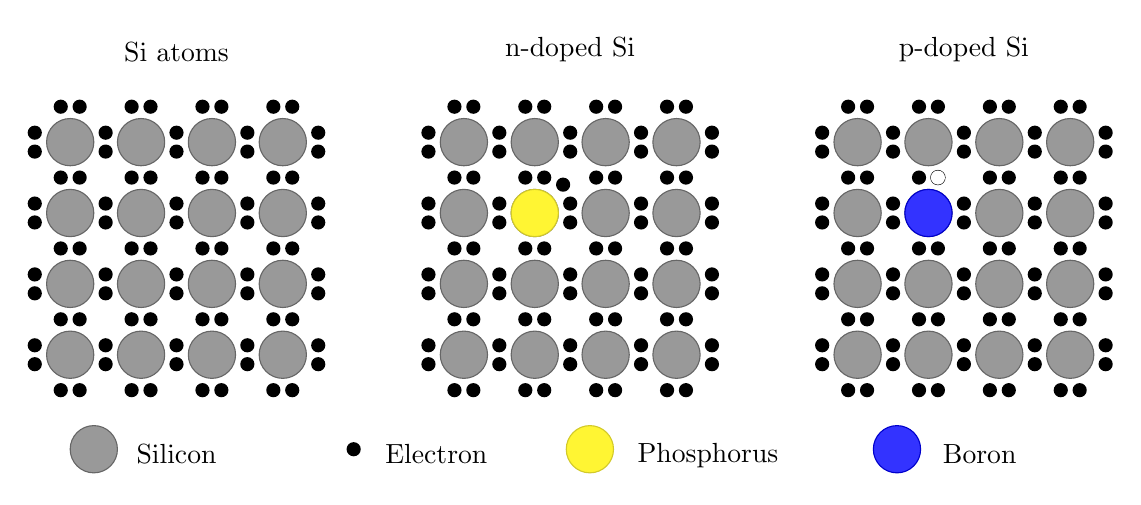
\begin{tikzpicture}

% Définition de l'objet
\newcommand{\myCircle}{
    \fill[gray!80] (0,0) circle (1);
    \draw[gray!80!black] (0,0) circle (1);
    
    \fill (-0.4,1.5) circle (0.3);
    \fill (0.4,1.5) circle (0.3);
    \fill (-1.5,0.4) circle (0.3);
    \fill (-1.5,-0.4) circle (0.3);
}

\newcommand{\LittleCircleRight}{
    \fill (1.5,0.4) circle (0.3);
    \fill (1.5,-0.4) circle (0.3);
}

\newcommand{\LittleCircleBottom}{
    \fill (-0.4,-1.5) circle (0.3);
    \fill (0.4,-1.5) circle (0.3);
}

\newcommand{\myYellowCircle}{
    \fill[yellow!80] (0,0) circle (1);
    \draw[yellow!80!black] (0,0) circle (1);
    
    \fill (1.2,1.2) circle (0.3);
}

\newcommand{\myBlueCircle}{
    \fill[blue!80] (0,0) circle (1);
    \draw[blue!80!black] (0,0) circle (1);
    
    \draw[black] (0.4,1.5) circle (0.3);
    \fill[white] (0.4,1.5) circle (0.3);
}


\newcommand{\SiliconLatice}{
    % Grille 4x4
    \foreach \i in {0,...,3} {
        \foreach \j in {0,...,3} {
            \begin{scope}[shift={({3*\i},{3*\j})}]
                \myCircle
                
                \ifnum\i=3
                    \LittleCircleRight 
                \fi
                
                \ifnum\j=0
                    \LittleCircleBottom
                \fi
            \end{scope}
        }
    }
}

\newcommand{\NLatice}{
    % Grille 4x4
    \foreach \i in {0,...,3} {
        \foreach \j in {0,...,3} {
            \begin{scope}[shift={({3*\i},{3*\j})}]
                \myCircle
                
                \ifnum\i=3
                    \LittleCircleRight 
                \fi

                \ifnum\j=2
                    \ifnum\i=1
                        \myYellowCircle
                    \fi
                \fi
                
                \ifnum\j=0
                    \LittleCircleBottom
                \fi
            \end{scope}
        }
    }
}

\newcommand{\PLatice}{
    % Grille 4x4
    \foreach \i in {0,...,3} {
        \foreach \j in {0,...,3} {
            \begin{scope}[shift={({3*\i},{3*\j})}]
                \myCircle
                
                \ifnum\i=3
                    \LittleCircleRight 
                \fi

                \ifnum\j=2
                    \ifnum\i=1
                        \myBlueCircle
                    \fi
                \fi
                
                \ifnum\j=0
                    \LittleCircleBottom
                \fi
            \end{scope}
        }
    }
}

\def\BlockStep{5}

\begin{scope}[shift={(0,0)}, scale=0.3]
    \node[above] at (4.5, 12) {Si atoms};
    \SiliconLatice
\end{scope}

\begin{scope}[shift={(\BlockStep,0)}, scale=0.3]
    \node[above] at (4.5, 12) {n-doped Si};
    \NLatice
\end{scope}

\begin{scope}[shift={(2*\BlockStep,0)}, scale=0.3]
    \node[above] at (4.5, 12) {p-doped Si};
    \PLatice
\end{scope}


% legend
\def\Ylegend{-4}

\begin{scope}[scale=0.3]
    \fill[gray!80] (1,\Ylegend) circle (1);
    \draw[gray!80!black] (1,\Ylegend) circle (1);

    \node[above] at (3+1.5, \Ylegend-1) {Silicon};
    
    \fill (12,\Ylegend) circle (0.3);
    \node[above] at (12+3.5, \Ylegend-1) {Electron};
    
    \fill[yellow!80] (22,\Ylegend) circle (1);
    \draw[yellow!80!black] (22,\Ylegend) circle (1);
    \node[above] at (27, \Ylegend-1.2) {Phosphorus};
    
    \fill[blue!80] (35,\Ylegend) circle (1);
    \draw[blue!80!black] (35,\Ylegend) circle (1);
    \node[above] at (35+3.5, \Ylegend-1) {Boron};
\end{scope}
    
\end{tikzpicture}}